% Shared float (common/make_floats.py). Figure: figures/cnn_curves.pdf
\begin{figure}[htbp]
\centering
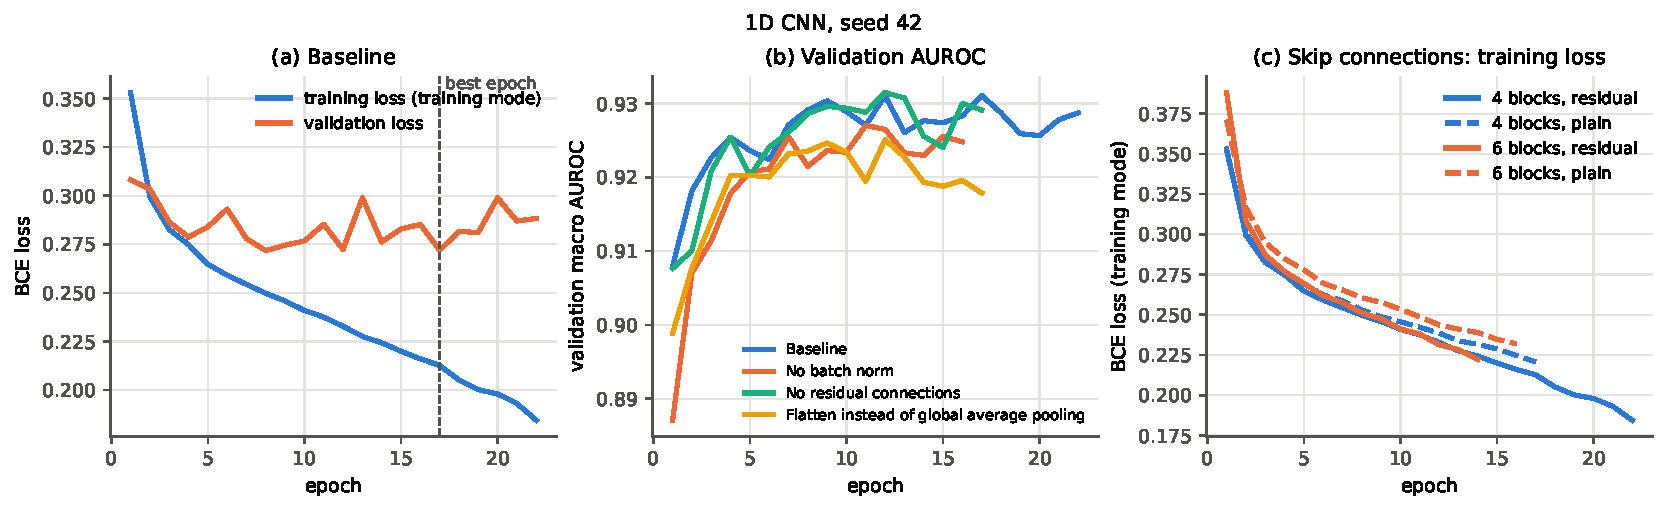
\includegraphics[width=\textwidth,height=0.42\textheight,keepaspectratio]{figures/cnn_curves.pdf}
\caption[1D CNN: learning curves]{1D CNN, seed 42. (a) Baseline training and validation loss; dashed line: best epoch. (b) Validation macro AUROC without batch norm, without residual connections and with flatten instead of global average pooling. (c) Training loss with and without residual connections, at 4 and 6 blocks.}
\label{fig:cnn_curves}
\end{figure}
